
\documentclass[a4paper,12pt]{article} % тип документа

% report, book

%  Русский язык

\usepackage[T2A]{fontenc}			% кодировка
\usepackage[utf8]{inputenc}			% кодировка исходного текста
\usepackage[english,russian]{babel}	% локализация и переносы
\usepackage{graphicx}                % Математика
\usepackage{amsmath,amsfonts,amssymb,amsthm,mathtools} 
\usepackage{mathtext}
\usepackage[T2A]{fontenc}
\usepackage[utf8]{inputenc}

\usepackage{wasysym}

%Заговолок
\author{Бичина Марина 
группа Б04-005 1 курса ФЭФМ}
\title{Отчет по лабораторной работе №2.1.6
Эффект Джоуля-Томсона}
\date{\today}


\begin{document} % начало документа


\section{Контрольные вопросы}
\begin{enumerate} 
\item Чем реальные газы отличаются от идеальных? \\ \\
В модели идеального газа не учитываются притяжение и отталкивание молекул газа между собой (потенциальная энергия). 

В реальных газах молекулы притягиваются на относительно больших расстояниях и отталкиваются вблизи, поэтому уравнение Менделеева-Клапейрона не точно описывает реальный газ и существуют более удачные модели (например, уравнение Ван-дер-Ваальса)

\item Начертите кривые, выражающие характер зависимости сил взаимодействия и взаимной потенциальной энергии двух молекул от расстояния между ними, и, используя их, объясните причины эффекта Джоуля-Томсона\\ \\
\begin{figure}[h]
\begin{minipage}[h]{0.49\linewidth}
\center{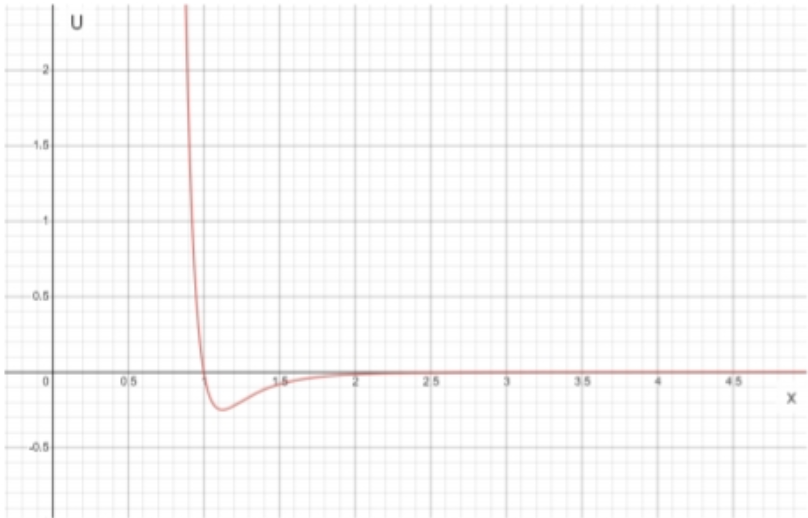
\includegraphics[width=0.7\linewidth]{lenard.png} \\ а)}
\end{minipage}
\hfill
\begin{minipage}[h]{0.49\linewidth}
\center{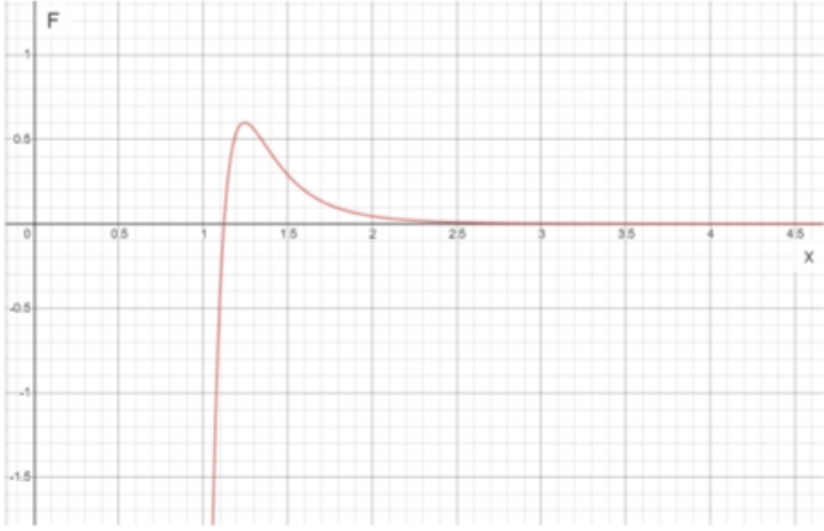
\includegraphics[width=0.7\linewidth]{potential.png} \\ б)}
\end{minipage}
\caption{а) -- Потенциал Леннарда-Джонса, б) -- Зависимость силы от расстояния между молекулами}
\label{ris:image1}
\end{figure}

В эффекте Джоуля-Томсона при идеальном газе  не изменяется температура, но при изменении объема реального газа влияет потенциальная энергия взаимодействия молекул между собой. Изменяется расстояние между молекулами и часть потенциальной энергии взаимодействия молекул переходит в энергию теплового движения и наоборот, то есть в температуру, которая изменяется (но, вроде, не должна была). 
PS Идеальный газ перешел в реальный

\item Какая температура называется критической? Что такое температура инверсии?\\ \\
Критической называется температура, изотерма которой является граничной между монотонными и волнобразными изотермами. Точка, в которой экстремумы изотерм сливаются
Температура инверсии -- это граничная температура, ниже которой газ охлаждается, а выше нагревается (для дифференциального эффекта Джоуля-Томсона)
\item Объясните качественно знак эффекта Джоуля томсона в случае
 
 1) $a = 0,b \not= 0$
 2) $a \not= 0,b = 0$\\ \\
 1) Газ всегда нагревается, поскольку соотношение всегда $(\Delta T/\Delta P)_H<0$ -- (соотношение $(\frac{\Delta T}{\Delta P})_H=\frac{1}{c_p * (dP/dV)_T}(\frac{bRT}{(V-b)^2}-\frac{2a}{V^2})$ для дифференциального эффекта Джоуля-Томсона)
\end{enumerate}
\section{Задачи от Жака Фреско}
\begin{enumerate}

\item  Физический смысл <<a>>, <<b>> \\ \\
Коэффициент b показывает запрещенный молекулам объем $b \simeq$ 4*(объем молекул в одном моле) = $N_AV_0$, поскольку молекулы -- не материальные точки, а <<шары>> радиуса r. Для эффекта Джоуля-Томсона b -- влияет на нагрев газа. Включает в себя силы отталкивания.

Коэффициент a учитывает притяжение молекул, например, через перераспределение зарядов внутри молекул и образование диполей. Для эффекта Джоуля-Томсона а -- влияет на охлажение газа. 
\item Чем отличается изотерма газа Ван-дер-Ваальса от изотермы реального газа и что описывают их разные участки.\\ \\
В отличие от случая идеального газа, некоторые изотермы газа Ван-дер-Ваальса ведут себя немонотонно. При одном и том же давлении вещество может обладать разным объемом. Для левой части$V < 3b$ -- соизмеримо с размером молекул => жидкость, для правой части $V > 3b$ - газ 

BD может быть реализовано только в неравновесном процессе и не может существовать неограниченно долго, т.к. состояние неустойчиво, поскольку не выполняется $(dP/dV)_T < 0$
\begin{figure}[h]
\center{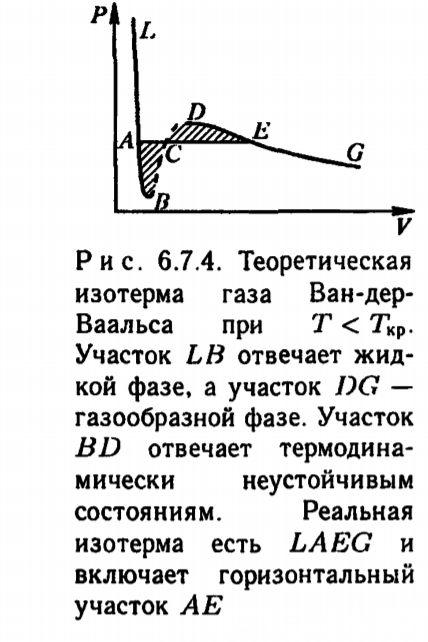
\includegraphics[width=0.36\linewidth]{VDV.png}}
\end{figure}
\item Что такое критическая точка?\\ \\ 
Выше есть
\item Доказательство что при адиабатическом дросселировании сохраняется энтальпия, и знать, что такое энтальпия.\\ \\
Энтальпия -- функция состояния термодинамической системы, равная $H = U + PV$. Для идеального газа $H = c_PT$


\end{enumerate}
\end{document}